% Provenance (never printed): see sources/outline_sources.md (Year 2: oceanic islands; growth,
% flank collapse and erosion of volcanic islands; reefs and atolls; subsidence). Hawaiian
% stages, slides, subsidence and drowned reefs after Clague and Sherrod (2014, USGS PP 1801
% ch. 3) and Denlinger and Morgan (2014, ch. 4); the Nuuanu slide after the ODP Leg 200 report;
% the Enewetak holes after Ladd and Schlanger (1960, USGS PP 260-Y); Kure after the NOAA
% monument pages; the depth--age law from the Book 2 and Book 3 rows. Curves and the invented
% Petrel island from figdata/bachelor-2/islands.py; exercise and problem values in the Book 4
% scratch calculator calc/ch17.py.
\chapter{महासागरीय द्वीप}\label{ch:b2:oceanic-islands}

1952 में, पश्चिमी प्रशांत के एनीवेटक \omterm{def:b2:oceanic-islands:reefs}{एटॉल} (तब एनिवेटोक लिखा जाता था) के दो द्वीपों पर, दो
बोरहोल प्रवाल-चट्टान के आर-पार \qty{1.2}{km} से अधिक गहराई तक गए। पैरी द्वीप पर, बरमा
4,158 फ़ुट, यानी \qty{1267}{m}, की गहराई पर ताज़े बेसाल्ट की कतरनें ऊपर लाया, और फिर
ओलिवीन बेसाल्ट का एक कोर। उसके ऊपर इओसीन आयु का चूना-पत्थर था, भित्ति-प्रवालों से भरा, ऐसी किस्म के जो
लगभग \qty{46}{m} से अधिक गहराई पर नहीं उगते। कभी एक प्रवाल-भित्ति समुद्र-तल के निकट किसी ज्वालामुखी के
कंधों पर उगी थी, और ज्वालामुखी एक किलोमीटर से अधिक धँस गया था जबकि भित्ति उसके ऊपर बढ़ती रही।
यह अध्याय किसी \omterm{def:b2:oceanic-islands:stages}{महासागरीय द्वीप} के पूरे जीवन का अनुसरण करता है: वह कैसे बढ़ता है, उसके पार्श्व
समुद्र में कैसे गिरते हैं, वह क्यों धँसता है, और प्रवाल का एक वलय उससे अधिक कैसे जी सकता है।
% ledger: ls60:enewetak, ics4:eocene

\begin{recall}
\textbf{पुस्तक 3 (स्नातक वर्ष 1) से}: हॉटस्पॉट, प्रावार-स्तंभ, हॉटस्पॉट-पथ और उसकी आयु-प्रगति,
हवाई--सम्राट शृंखला और हवाई उभार; महासागर-तल का गहराई–आयु नियम; भित्तियाँ,
डार्विन द्वारा वर्णित उनके तटीय, अवरोधक और \omterm{def:b2:oceanic-islands:reefs}{एटॉल} रूप, और नियम ``ऊपर उठो या
डूबो''; यूस्टेसी और अंतिम हिमनदीय अधिकतम का समुद्र-स्तर, जो आज से लगभग \qty{120}{m}
नीचा था। \textbf{स्कूल की पुस्तकों से}: शील्ड ज्वालामुखी; तरंग-घर्षित चबूतरा।
\textbf{\cref{ch:b2:magmatic-series} से}: थोलिआइटी और \omterm{def:b2:magmatic-series:series}{क्षारीय श्रेणियाँ}।
\end{recall}

\section{ज्वालामुखी द्वीप का विकास}\label{sec:b2:oceanic-islands:growth}

हवाई द्वीप उस शृंखला का सबसे नया छोर हैं जिसका अनुसरण पुस्तक 3 ने उत्तरी प्रशांत के
आर-पार किया था। मुख्य द्वीपों में 19 ज्ञात शील्ड ज्वालामुखी हैं: 15 समुद्र से ऊपर खड़े हैं,
3 जलमग्न हैं, और एक, नवजात, अब भी पानी के नीचे है। जैसे-जैसे प्रशांत प्लेट उन्हें
उत्तर-पश्चिम की ओर ले जाती है, हर एक हॉटस्पॉट के ऊपर जन्मता है, बढ़ता है, दूर खिसकते हुए मरता है, और धँसता है। यह जीवन
इतना नियमित है कि उसे चरणों में बाँटा जा सकता है।
% ledger: cs14:volcanoes

\begin{definition}[महासागरीय द्वीप; विकास के चरण]\label{def:b2:oceanic-islands:stages}
\emph{महासागरीय द्वीप}\index{महासागरीय द्वीप} वह ज्वालामुखी द्वीप है जो महासागर-तल से
उठता है और महासागरीय स्थलमंडल पर बना होता है। किसी हॉटस्पॉट शृंखला का द्वीप चार उद्गारी
चरणों से गुज़रता है: समुद्र-तल पर क्षारीय लावा के छोटे उद्गारों वाला \emph{पूर्व-शील्ड} चरण;
\emph{शील्ड चरण}\index{शील्ड चरण}, जिसमें थोलिआइटी लावा ज्वालामुखी का अधिकांश भाग बनाता है
जब तक वह हॉटस्पॉट के ऊपर रहता है; कम और अधिक क्षारीय उद्गारों वाला \emph{उत्तर-शील्ड} चरण,
जो शील्ड को ढक देते हैं; और, एक विराम के बाद, दुर्लभ, छोटे क्षारीय उद्गारों वाला \emph{पुनर्जीवित}
चरण। फिर अपरदन और धँसाव का काम शुरू होता है।
\end{definition}
% ledger: usgs14:hawaii-stages, cs14:rejuvenated

चरण ऊष्मा की आपूर्ति का अनुसरण करते हैं। सबसे नया ज्वालामुखी लोइही किलाउआ के शिखर से \qty{54}{km}
दक्षिण में है; उसका शीर्ष अब भी समुद्र के \qty{975}{m} नीचे है पर अपने आसपास के समुद्र-तल से पहले ही \qty{2.5}{km}
ऊपर है, और उसके सबसे पुराने लावा क्षारीय हैं। \omterm{def:b2:oceanic-islands:stages}{शील्ड चरण} में ज्वालामुखी
हॉटस्पॉट के ऊपर रहता है और सबसे ऊँची दर से पोषित होता है। हर हवाई ज्वालामुखी अपने अंतिम आयतन का अनुमानतः 80 से
\qty{95}{\percent} इसी चरण में उगलता है, अधिकांशतः अपने पहले 1 से \qty{2}{Myr} के भीतर।
चरण के अंत में उद्गार की दर दस गुना गिर जाती है। उथले मैग्मा-भंडार, 1
से \qty{7}{km} गहरे, अब जीवित नहीं रखे जा सकते, यद्यपि 20 से \qty{30}{km} पर छोटे भंडार
बने रहते हैं। लावा फिर क्षारीय हो जाता है, क्योंकि गलन की निम्नतर मात्रा उसे ऐसा बनाती है, जैसा
\cref{ch:b2:magmatic-series} ने दिखाया। पुनर्जीवित चरण 0.5 से कम
से \qty{2.0}{Myr} तक के विराम के बाद आता है। वह एक या दो प्रकरण हो सकता है, या बहुत लंबा: निहाउ पर वह 2.2 से
\qty{0.4}{Ma} तक चला, और काउआई पर वह \qty{3.5}{Ma} से जारी है।
% ledger: cs14:loihi, usgs14:hawaii-stages, cs14:rejuvenated

आयतन विशाल हैं। माउना लोआ का आयतन लगभग \qty{74000}{km^3} आँका गया है। जब किलाउआ के साथ उसकी सीमा फिर से इस तरह खींची जाती है कि किलाउआ के पास केवल लगभग
\qty{10000}{km^3} रहे, तो माउना लोआ का हिस्सा बढ़कर \qty{95600}{km^3} हो जाता है। युवा लोइही में
\qty{1700}{km^3} है। पूरी शृंखला, \qty{81}{Ma} से, लगभग
\qty{2e6}{km^3} की है; उस इतिहास पर समाकलित उद्गार-दर, प्रति वर्ष \qty{0.07}{km^3}, लगभग तीन गुना देती। भार इतना भारी है कि वह
प्लेट को झुका देता है: द्वीपों के नीचे की महासागरीय भूपर्पटी \qty{5}{km} तक नीचे दबी है, एक
द्रोणिका के अनुदिश जिसे हवाई परिखा (मोट) कहते हैं, और कुछ सौ किलोमीटर दूर एक नीचा उभार, हवाई मेहराब,
उठता है। कोई प्लेट किसी भार के नीचे कैसे झुकती है, यह पुस्तक~5 में लिया गया है। यहाँ परिखा
इसलिए महत्त्वपूर्ण है क्योंकि द्वीपों का अधिकांश मलबा वहीं पहुँचता है।
% ledger: cs14:volumes, cs14:loihi, cs14:moat

\begin{omfigure}
\centering
\begin{tikzpicture}[x=0.95cm, y=0.95cm, font=\footnotesize]
% schematic, not to scale (vertical exaggeration about 10). Sea level y = 0; sea floor
% y = -1.6 - 0.0625 (16 - x), deepening with the age of the plate to the left.
\fill[omSea!45] (0,0) -- (16,0) -- (16,-1.6) -- (0,-2.6) -- cycle;
\fill[black!18] (0,-2.6) -- (16,-1.6) -- (16,-3.1) -- (0,-3.1) -- cycle;
\draw[black!60] (0,-2.6) -- (16,-1.6);
\draw[omSea!60!black] (0,0) -- (16,0);
\node[anchor=south, font=\scriptsize] at (8.7,0) {समुद्र-तल};
% (a) shield stage over the hotspot
\fill[lith basalt, draw=black!70] (12.6,-1.8125) -- (13.9,0.75) -- (14.3,0.9) -- (14.7,0.75) -- (16,-1.6) -- cycle;
% (b) eroded island with a fringing reef (valleys notched in the summit)
\fill[lith basalt, draw=black!70] (9.2,-2.025) -- (10.1,0.15) -- (10.3,0.35) -- (10.45,0.2) -- (10.6,0.45) -- (10.8,0.25) -- (11.0,0.3) -- (11.2,0.1) -- (12.0,-1.85) -- cycle;
\fill[lith reef limestone, draw=black!70] (10.038,0) -- (9.976,-0.15) -- (9.80,0) -- cycle;
\fill[lith reef limestone, draw=black!70] (11.241,0) -- (11.303,-0.15) -- (11.46,0) -- cycle;
% (c) barrier reef around a smaller island, a lagoon between
\fill[lith basalt, draw=black!70] (5.8,-2.2375) -- (7.0,0.2) -- (8.2,-2.0875) -- cycle;
\fill[lith reef limestone, draw=black!70] (6.384,-1.05) -- (6.42,0) -- (6.60,0) -- (6.62,-0.45) -- (6.680,-0.45) -- cycle;
\fill[lith reef limestone, draw=black!70] (7.656,-1.05) -- (7.62,0) -- (7.44,0) -- (7.42,-0.45) -- (7.341,-0.45) -- cycle;
% (d) atoll: volcano bevelled and drowned, reef cap with a lagoon
\fill[lith basalt, draw=black!70] (2.7,-2.43125) -- (3.6,-0.55) -- (4.0,-0.55) -- (4.9,-2.29375) -- cycle;
\fill[lith reef limestone, draw=black!70] (3.4325,-0.9) -- (3.47,0) -- (4.14,0) -- (4.1806,-0.9) -- (4.0,-0.55) -- (3.6,-0.55) -- cycle;
\fill[omSea!45] (3.62,-0.15) rectangle (3.99,0);
% (e) guyot: flat top with a drowned reef cap, beyond the Darwin point
\fill[lith basalt, draw=black!70] (0.2,-2.5875) -- (0.9,-0.95) -- (1.7,-0.95) -- (2.4,-2.475) -- cycle;
\fill[lith reef limestone, draw=black!70] (0.9,-0.95) -- (0.96,-0.75) -- (1.64,-0.75) -- (1.7,-0.95) -- cycle;
% Darwin point
\draw[black!70, dashed] (2.55,0.55) -- (2.55,-2.5);
\node[anchor=south, font=\scriptsize] at (2.55,0.55) {डार्विन बिंदु};
% hotspot and plate motion
\draw[omThm, line width=1.4pt, -{Stealth[length=2.5mm]}] (14.3,-3.9) -- (14.3,-3.15);
\node[anchor=west, font=\scriptsize, text=omThm] at (14.4,-3.7) {हॉटस्पॉट};
\draw[black, line width=0.8pt, -{Stealth[length=2.5mm]}] (9.5,-2.85) -- (6.5,-2.85);
\node[anchor=west, font=\scriptsize] at (9.6,-2.85) {प्लेट की गति};
\node[anchor=west, font=\scriptsize] at (0.1,-2.9) {महासागरीय स्थलमंडल};
% stage labels
\node[align=center, font=\scriptsize] at (14.3,1.45) {(क) शील्ड चरण};
\node[align=center, font=\scriptsize] at (10.6,1.3) {(ख) अपरदित द्वीप,\\ तटीय भित्ति};
\node[align=center, font=\scriptsize] at (7.0,1.45) {(ग) अवरोधक भित्ति};
\node[align=center, font=\scriptsize] at (3.8,1.45) {(घ) एटॉल};
\node[align=center, font=\scriptsize] at (1.3,1.45) {(ङ) गयो};
\draw[black!60, -{Stealth[length=2mm]}] (13.6,-3.7) -- (0,-3.7);
\node[anchor=south, font=\scriptsize, fill=white, inner sep=1pt] at (7,-3.7) {पुराने ज्वालामुखी, पुरानी और गहरी प्लेट};
\end{tikzpicture}
\par\smallskip{\small किसी हॉटस्पॉट शृंखला के अनुदिश पढ़ा गया एक \omterm{def:b2:oceanic-islands:stages}{महासागरीय द्वीप} का जीवन (योजनामूलक, पैमाने
के बिना, ऊर्ध्वाधर पैमाना बहुत बढ़ाकर)। प्लेट हर ज्वालामुखी को हॉटस्पॉट (दाएँ) से दूर ले जाती है
और ज्वालामुखी उसके साथ धँसता है, जबकि अपरदन उसे घिसता है। (क)~हॉटस्पॉट के ऊपर एक शील्ड ज्वालामुखी
बढ़ता है। (ख)~विलुप्त और अपरदित, वह भित्तियों से घिरा है। (ग)~और धँसने पर, वह
एक \omterm{def:b2:oceanic-islands:reefs}{अवरोधक भित्ति} से घिरा है जिसके पीछे एक लैगून है। (घ)~उसका शिखर समुद्र के नीचे जा चुका है, और उसके ऊपर
एक केंद्रीय लैगून वाली भित्ति-टोपी, एक \omterm{def:b2:oceanic-islands:reefs}{एटॉल}, उगती है। (ङ)~भित्ति के बढ़ते रहने के लिए बहुत ठंडे पानी में ले जाए जाने पर
\omterm{def:b2:oceanic-islands:reefs}{एटॉल} डूब जाता है और एक सपाट-शीर्ष \omterm{def:b2:oceanic-islands:seamount}{गयो} के रूप में धँसता है।}
\end{omfigure}
% ledger: cs14:volcanoes, cs14:erase, cs14:darwin-point, pmnm:geology

\section{पार्श्व-ढहन}\label{sec:b2:oceanic-islands:collapse}

कई किलोमीटर ऊँचा ज्वालामुखी, जो ढीले लावा-प्रवाहों और मलबे से बना है और ऐसी ढलानों पर खड़ा है जो
परिखा में नीचे उतरती हैं, स्थिर नहीं होता। 1975 में 7.7 परिमाण के कालापाना भूकंप ने
किलाउआ के दक्षिणी पार्श्व को एक ही झटके में समुद्र की ओर \qty{10}{m} तक खिसका दिया और एक सुनामी उठाई।
1868 में, एक और पार्श्व-गति 7.9 परिमाण के भूकंप और एक सुनामी के साथ आई, जिसने 46
लोगों की जान ली। इन पार्श्वों के नीचे भूकंपीय प्रोफ़ाइल एक गहरा परावर्तक दिखाते हैं। उसे
पुरानी महासागरीय भूपर्पटी के शीर्ष के अनुदिश एक \omterm{def:b2:alpine-orogen:decollement}{डेकोलमां} माना जाता है, जिस पर पूरा पार्श्व सरकता है। सामान्यतः
पार्श्व रेंगता है; कभी-कभी वह टूट जाता है।
% ledger: dm14:flank

\begin{definition}[पार्श्व-ढहन; मलबा-हिमस्खलन; स्लंप]\label{def:b2:oceanic-islands:collapse}
\emph{पार्श्व-ढहन}\index{पार्श्व-ढहन} किसी ज्वालामुखी के पार्श्व के एक बड़े भाग का विफल होना है,
जो अपने ही भार से सरक जाता है। जब गतिशील द्रव्यमान टूटकर तेज़ी से
बहता है, खंडों और मलबे के एक प्रवाह के रूप में जो ज्वालामुखी के पाद से बहुत आगे तक जा सकता है, तो वह
\emph{मलबा-हिमस्खलन}\index{मलबा-हिमस्खलन} है। जब वह धीरे-धीरे चलता है, बड़े खंडों के रूप में जो किसी गहरे \omterm{def:b2:alpine-orogen:decollement}{डेकोलमां} में
जड़ित भ्रंशों पर घूमते हैं और ज्वालामुखी के निकट ही रहते हैं, तो वह \emph{स्लंप} है।
\end{definition}

प्रमाण समुद्र के नीचे हैं। 1980 के दशक के अंत में, हवाई द्वीपों के आसपास के जल के साइडस्कैन सोनार
मानचित्रण ने गहरे समुद्र-तल पर, द्वीपों से कई सौ किलोमीटर दूर तक, बिखरा मलबा
और बड़े खंडित ब्लॉकों से बने स्लंप दिखाए। मुख्य द्वीपों के आसपास सत्रह बड़े स्खलन पहचाने गए,
जो पिछले \qty{5}{Myr} में बने। अब हवाई द्वीप और मिडवे के बीच हवाई कटक के अनुदिश सत्तर ज्ञात हैं,
जो \qty{30}{Myr} में बने। यानी मुख्य द्वीपों के आसपास हर \qty{300}{kyr} में कम से कम
एक स्खलन। ये गणनाएँ न्यूनतम हैं, क्योंकि कोई नया ज्वालामुखी किसी पुराने का निशान और मलबा दबा सकता है:
निहाउ का शिखर काल्डेरा और एक दरार-क्षेत्र गायब हैं, और उनके लिए कोई निक्षेप नहीं मिला है। विशाल स्खलन तब
सबसे अधिक संभावित लगते हैं जब ज्वालामुखी सबसे तेज़ी से बढ़ता
है, पूर्व-शील्ड चरण के अंत से उत्तर-शील्ड चरण के आरंभ तक, पर वे
उसके बहुत बाद तक जारी रहते हैं।
% ledger: cs14:slides, dm14:flank

सबसे बड़ा नुउआनु भूस्खलन है, जिसने ओआहू पर कूलाउ ज्वालामुखी के उत्तर-पूर्वी पार्श्व को
उखाड़ दिया। यह \qty{23000}{km^2} पर फैला एक \omterm{def:b2:oceanic-islands:collapse}{मलबा-हिमस्खलन} है, जो द्वीप से
\qty{200}{km} से अधिक दूर तक जाता है। इसके खंडों में टस्कलूसा \omterm{def:b2:oceanic-islands:seamount}{समुद्री पर्वत} है, लगभग \qty{30}{km} लंबा,
\qty{17}{km} चौड़ा और कम से कम \qty{2}{km} ऊँचा। हिमस्खलन ने गहरी परिखा पार की और
हवाई मेहराब की ढलान पर \qty{100}{km} से अधिक ऊपर चढ़ा। इसकी आयु 2.1 से
\qty{1.8}{Ma} आँकी गई है, कूलाउ के जीवन के अंत के निकट या उसके बाद, जिसके सतही लावा 1.8 से
\qty{2.6}{Ma} पुराने हैं। यह कितने ढहनों से बना था, और द्वीप से दूर यह कितना मोटा है,
ये प्रश्न अब भी खुले हैं।
% ledger: odp200:nuuanu

\begin{omfigure}
\centering
\begin{tikzpicture}[x=0.95cm, y=0.95cm, font=\footnotesize]
% schematic section from the summit of an island (left) across the moat to the arch (right);
% not to scale. Sea level y = 0; top of the old oceanic crust, bent down under the island.
\fill[omSea!45] (0,0) -- (15,0) -- (15,-2.2) -- (13.5,-2.12) -- (11,-2.05) -- (8.5,-2.35) -- (6.5,-2.75) -- (5.6,-2.82) -- (4.0,-1.4) -- (2.5,0) -- cycle;
\fill[black!18] (0,-3.05) -- (5.6,-2.82) -- (6.5,-2.75) -- (8.5,-2.35) -- (11,-2.05) -- (13.5,-2.12) -- (15,-2.2) -- (15,-3.6) -- (0,-3.6) -- cycle;
\draw[black!70] (0,-3.05) -- (5.6,-2.82) -- (6.5,-2.75) -- (8.5,-2.35) -- (11,-2.05) -- (13.5,-2.12) -- (15,-2.2);
\draw[omSea!60!black] (0,0) -- (15,0);
\node[anchor=south east, font=\scriptsize] at (15,0) {समुद्र-तल};
% the volcano: present flank (after collapse) and the lost flank (dashed)
\fill[lith basalt, draw=black!70] (0,1.15) -- (0.8,1.05) -- (1.25,0.95) -- (1.45,0.45) -- (1.75,0.1) -- (2.6,-0.75) -- (3.6,-1.6) -- (4.6,-2.4) -- (5.6,-2.82) -- (0,-3.05) -- cycle;
\draw[black!70, dashed] (1.25,0.95) -- (2.5,0) -- (4.0,-1.4) -- (5.6,-2.82);
\node[font=\scriptsize, align=center, fill=white, inner sep=1pt] at (0.8,-1.6) {ज्वालामुखी};
\node[font=\scriptsize, anchor=south west, align=left] at (2.0,0.25) {खोए पार्श्व\\ का निशान};
% slump: blocks rotated on listric faults rooted in the decollement
\draw[black, line width=0.7pt] (1.45,0.45) .. controls (1.7,-1.4) and (2.4,-2.6) .. (3.6,-2.95);
\draw[black, line width=0.7pt] (2.6,-0.75) .. controls (2.8,-1.8) and (3.3,-2.6) .. (4.4,-2.9);
\draw[omThm, line width=1.1pt] (0.6,-3.03) -- (5.6,-2.82);
\node[anchor=north, font=\scriptsize, text=omThm] at (2.9,-3.05) {डेकोलमां};
% debris avalanche: hummocky sheet across the moat and up the arch, with blocks
\fill[lith conglomerate, draw=black!70] (4.6,-2.4) -- (5.6,-2.62) -- (6.5,-2.6) -- (8.5,-2.22) -- (11,-1.95) -- (12.6,-2.03) -- (11,-2.05) -- (8.5,-2.35) -- (6.5,-2.75) -- (5.6,-2.82) -- cycle;
\fill[lith basalt, draw=black!70] (7.0,-2.62) -- (7.25,-2.25) -- (7.95,-2.22) -- (8.1,-2.43) -- cycle;
\fill[lith basalt, draw=black!70] (9.3,-2.2) -- (9.45,-2.02) -- (9.75,-2.0) -- (9.85,-2.17) -- cycle;
\fill[lith basalt, draw=black!70] (10.6,-2.05) -- (10.7,-1.93) -- (10.9,-1.92) -- (10.95,-2.03) -- cycle;
\draw[black!70] (7.6,-2.2) -- (7.4,-1.3) node[anchor=south, font=\scriptsize, align=center] {कई km चौड़ा\\ खंड};
\node[anchor=south, font=\scriptsize, align=center] at (10.3,-1.3) {मलबा-हिमस्खलन};
\draw[black!70] (10.3,-1.3) -- (10.0,-1.98);
\node[font=\scriptsize] at (6.6,-3.2) {परिखा};
\node[font=\scriptsize] at (11.6,-2.6) {मेहराब};
\node[anchor=west, font=\scriptsize] at (12.6,-3.3) {महासागरीय भूपर्पटी};
\draw[black!70] (2.55,-1.55) -- (3.35,-0.6) node[anchor=west, font=\scriptsize, inner sep=1pt] {स्लंप};
\draw[black!60, {Stealth[length=2mm]}-{Stealth[length=2mm]}] (5.6,-3.95) -- (12.6,-3.95);
\node[anchor=north, font=\scriptsize] at (9.1,-3.95) {लगभग \qty{200}{km} तक};
\end{tikzpicture}
\par\smallskip{\small किसी \omterm{def:b2:oceanic-islands:stages}{महासागरीय द्वीप} का \omterm{def:b2:oceanic-islands:collapse}{पार्श्व-ढहन} (योजनामूलक, पैमाने के बिना)। ज्वालामुखी के
निकट, एक स्लंप घूमते खंडों के रूप में उन भ्रंशों पर धीरे-धीरे चलता है जो पुरानी महासागरीय भूपर्पटी के शीर्ष पर
एक \omterm{def:b2:alpine-orogen:decollement}{डेकोलमां} में जड़ित हैं। एक \omterm{def:b2:oceanic-islands:collapse}{मलबा-हिमस्खलन} पार्श्व से टूटकर एक निशान छोड़ता है, और
कई किलोमीटर चौड़े खंडों को ढोती मलबे की एक चादर के रूप में बहता है। नुउआनु हिमस्खलन ने परिखा पार की
और मेहराब पर चढ़ा, ओआहू से \qty{200}{km} से अधिक दूर।}
\end{omfigure}
% ledger: dm14:flank, odp200:nuuanu, cs14:moat

समुद्र में गिरता स्खलन पानी को एक ओर धकेलता है। लानाई और मोलोकाई पर, प्रवाल और लावा की अव्यवस्थित संकोणाश्म
समुद्र-तल से \qty{155}{m} तक ऊपर खड़ी हैं और उन्हें ढहनों से उठी
विशाल लहरों के निक्षेप माना गया है। यह व्याख्या विवादित है। कुछ लेखक निक्षेपों की व्याख्या द्वीपों के
उत्थान से करते हैं, यद्यपि लानाई के दक्षिण की डूबी भित्तियाँ ऐसे उत्थान का कोई संकेत नहीं दिखातीं।
विशाल हवाई स्खलनों में से लगभग एक तिहाई विशाल लहरें उठाने में सक्षम \omterm{def:b2:oceanic-islands:collapse}{मलबा-हिमस्खलन} थे। ऐसे
दुर्लभ पर बहुत बड़े संकट को कैसे तौला जाता है, यह \cref{ch:b2:geological-hazards} का प्रश्न है।
% ledger: cs14:megatsunami

\section{महासागरीय द्वीप क्यों धँसते हैं}\label{sec:b2:oceanic-islands:subsidence}

दो प्रक्रियाएँ किसी \omterm{def:b2:oceanic-islands:stages}{महासागरीय द्वीप} को धँसाती हैं, और वे एक-दूसरे पर चढ़ी होती हैं। पहली भारण है: जैसे-जैसे ज्वालामुखी
बढ़ता है, उसका भार प्लेट को नीचे दबाता है। यह तीव्र चरण शायद दस लाख वर्ष चलता है और
तटरेखाओं और भित्तियों को एक किलोमीटर से अधिक डुबो देता है। हवाई द्वीप के उत्तर-पश्चिमी तट के पास,
तिथि-निर्धारित डूबी भित्तियाँ प्रति हज़ार वर्ष \qty{2.6}{m} की धँसाव-दर देती हैं। एक छोटा
ज्वालामुखी इस चरण में पूरी तरह डूब सकता है: हवाई द्वीप के पास माहुकोना कुछ समय के लिए एक
द्वीप था और अब उसका शिखर पानी के नीचे लगभग \qty{1100}{m} पर है। दूसरी प्रक्रिया प्लेट का
शीतलन है, जो सौ मिलियन वर्ष तक चलता है, और जिसे यह अनुभाग
संख्याओं में रखता है।
% ledger: cs14:subsidence, cs14:mahukona

पुस्तक 3 ने मापा था कि महासागर-तल अपनी आयु $t$ (\unit{Myr} में) के साथ कैसे गहरा होता है। इस
अध्याय में प्रयुक्त रूप में:
\[
d(t) = \qty{2500}{m} + C\sqrt{t}, \qquad C = \qty{350}{m.Myr^{-1/2}}, \qquad 0 \le t \le 70,
\]
और, लगभग \qty{20}{Myr} से पुरानी प्लेटों के लिए,
\[
d(t) = \qty{6400}{m} - \qty{3200}{m}\; e^{-t/62.8}.
\]
दोनों रूप लगभग \qty{20}{m} के भीतर मेल खाते हैं, 20 और \qty{50}{Myr} के बीच, और
\qty{26}{Myr} पर एक-दूसरे को काटते हैं।
% ledger: ps77:depth-age (Book 2), parsons:plate-model (Book 3)
% values (islands.py): t_switch 26.27, d_switch 4293.8; root - exp: 20 Myr -7.6, 50 Myr +18.3

\begin{proposition}[द्वीप का तापीय धँसाव]\label{prop:b2:oceanic-islands:sinking}
आयु $t_1$ की प्लेट पर बना द्वीप, जो प्लेट के साथ ढोया जाता है, उसे एक ऐसे भार से भारित करता है जो
अब नहीं बदलता, और अपने नीचे प्लेट के शीतलन को अपरिवर्तित छोड़ता है, धँसता है
\[
S = d(t_2) - d(t_1)
\]
जब तक प्लेट आयु $t_2$ तक पहुँचती है, दर $\dot S = d'(t)$ से। मूल नियम के साथ,
\[
S = C\left(\sqrt{t_2} - \sqrt{t_1}\right), \qquad \dot S = \frac{C}{2\sqrt t},
\]
और, घातांकी नियम के साथ, $\dot S = (\qty{3200}{m}/\qty{62.8}{Myr})\,e^{-t/62.8}$। किसी
दिए गए अंतराल में, युवा प्लेट अपने द्वीपों को पुरानी प्लेट से अधिक नीचे ले जाती है।
\end{proposition}

\begin{proof}
प्लेट के एक ही आयु के दो स्तंभों की तुलना कीजिए, एक द्वीप के नीचे और एक दूर खुले
महासागर के नीचे। दोनों एक ही तरह ठंडे होते हैं, क्योंकि द्वीप प्लेट के शीतलन को अपरिवर्तित छोड़ता है। अतः दोनों समान मात्रा में सिकुड़ते हैं, और हर एक का शीर्ष समान
मात्रा में नीचे जाता है। द्वीप का अपना भार पहले से संतुलित है और अब नहीं बदलता, इसलिए वह कुछ
और नहीं जोड़ता। खुले महासागर का स्तंभ $d(t_2) - d(t_1)$ नीचे जाता है; द्वीप भी। अवकलन करने पर
दर मिलती है। अंतिम दावे के लिए: किसी नियत अंतराल $\Delta$ में, $C(\sqrt{t_1 + \Delta} -
\sqrt{t_1})$ $t_1$ के बढ़ने पर घटता है, क्योंकि उसका अवकलज, $\frac C2\bigl(1/\sqrt{t_1 + \Delta}
- 1/\sqrt{t_1}\bigr)$, ऋणात्मक है।
\end{proof}

प्रस्ताव जान-बूझकर दो बातें छोड़ देता है। हॉटस्पॉट का उभार प्लेट को गुज़रते समय
ऊपर उठाता है और दूर जाते समय फिर नीचे आने देता है, जो सबसे नए द्वीपों के धँसाव में जुड़ता है
(पुस्तक 3 ने उभार मापा था)। और ज्वालामुखी के बढ़ते समय भार बदलता है, जो ऊपर का
तीव्र चरण है। दोनों के समाप्त होने पर, द्वीप तल का अनुसरण करता है।

दरें छोटी हैं। \qty{4}{Myr} पुरानी प्लेट पर, मूल नियम प्रति मिलियन वर्ष \qty{87.5}{m}
देता है, यानी प्रति वर्ष एक मिलीमीटर के दसवें भाग से कम। \qty{100}{Myr} पुरानी प्लेट पर, घातांकी
नियम प्रति मिलियन वर्ष \qty{10.4}{m} देता है, यानी प्रति हज़ार वर्ष \qty{0.01}{m}। यही वह दर है
जो हवाई कटक और सम्राट \omterm{def:b2:oceanic-islands:seamount}{समुद्री पर्वतों} के अधिकांश भाग के अनुदिश मापी गई है। भारण चरण,
प्रति हज़ार वर्ष \qty{2.6}{m} पर, कोई 250 गुना तेज़ है।
% ledger: cs14:subsidence; values (islands.py): rate_100 10.37, age_rate10 102.3

\begin{omfigure}
\centering
% figdata/bachelor-2/islands.py part sink
\begin{tikzpicture}
\begin{axis}[width=0.8\linewidth, height=6.2cm, y dir=reverse, xmin=0, xmax=100, ymin=0,
  ymax=3000, xlabel={द्वीप बनने के बाद का समय (\unit{Myr})},
  ylabel={तापीय धँसाव (\unit{m})}, tick label style={font=\scriptsize},
  label style={font=\small}, xtick pos=bottom, ytick pos=left]
\addplot[omThm, line width=1pt] table[x=dt_Myr, y=t2] {figdata/out/bachelor-2-islands-sink.dat};
\addplot[orange!80!black, line width=1pt] table[x=dt_Myr, y=t10] {figdata/out/bachelor-2-islands-sink.dat};
\addplot[blue!70!black, line width=1pt] table[x=dt_Myr, y=t30] {figdata/out/bachelor-2-islands-sink.dat};
\addplot[black!45, line width=1pt] table[x=dt_Myr, y=t60] {figdata/out/bachelor-2-islands-sink.dat};
\node[font=\scriptsize, anchor=south east, inner sep=1pt] at (axis cs:99,2470) {\qty{2}{Myr} पुरानी प्लेट};
\node[font=\scriptsize, anchor=south east, inner sep=1pt] at (axis cs:99,2140) {\qty{10}{Myr}};
\node[font=\scriptsize, anchor=south east, inner sep=1pt] at (axis cs:99,1380) {\qty{30}{Myr}};
\node[font=\scriptsize, anchor=south east, inner sep=1pt] at (axis cs:99,710) {\qty{60}{Myr}};
\draw[black!50, dashed] (axis cs:0,1267) -- (axis cs:58,1267);
\node[font=\scriptsize, anchor=north west, inner sep=1pt] at (axis cs:1,1300) {एनीवेटक, \qty{1267}{m}};
\end{axis}
\end{tikzpicture}
\par\smallskip{\small प्लेट द्वारा ढोए गए द्वीप का तापीय धँसाव, गहराई–आयु नियम से,
2, 10, 30 और \qty{60}{Myr} पुरानी प्लेटों पर बने द्वीपों के लिए (प्लेट-आयु
\qty{26}{Myr} तक मूल नियम, उसके आगे घातांकी नियम, जहाँ दोनों मिलते हैं)। प्लेट जितनी युवा, द्वीप उतनी तेज़ी से
और उतना अधिक धँसता है। धराशायी रेखा एनीवेटक के नीचे बेसाल्ट की गहराई अंकित करती है, यानी
भित्ति-चट्टान की वह मोटाई जिसके लिए धँसाव को जगह बनानी होती है।}
\end{omfigure}
% ledger: ps77:depth-age (Book 2), parsons:plate-model (Book 3), ls60:enewetak

\section{भित्तियाँ, एटॉल और गयो}\label{sec:b2:oceanic-islands:reefs}

पुस्तक 3 ने भित्ति के तीन रूपों का वर्णन डार्विन की व्याख्या के अनुसार किया था, किसी द्वीप से सटी भित्ति से
लैगून के चारों ओर प्रवाल के वलय तक, और एक प्रश्न पर समाप्त किया था: द्वीप क्यों धँसते हैं,
और कितना? पिछले अनुभाग ने उसका उत्तर दिया। अब रूपों को नीचे के द्वीप की अवस्था से
परिभाषित किया जा सकता है।

\begin{definition}[तटीय भित्ति; अवरोधक भित्ति; एटॉल]\label{def:b2:oceanic-islands:reefs}
\emph{तटीय भित्ति}\index{तटीय भित्ति} किसी द्वीप के तट से जुड़ी भित्ति है, जिनके बीच कोई
लैगून नहीं होता, या केवल एक सँकरी, उथली नाली होती है। \emph{अवरोधक भित्ति}\index{अवरोधक भित्ति}
तट से एक लैगून द्वारा अलग भित्ति है, किसी ऐसे द्वीप के पार्श्वों पर जो धँसा है जबकि
भित्ति ऊपर की ओर बढ़ी। \emph{एटॉल}\index{एटॉल} भित्ति का एक वलय है, भित्ति-मलबे के निचले द्वीपों के साथ,
ऐसे लैगून के चारों ओर जिसमें समुद्र-तल से ऊपर कोई ज्वालामुखीय चट्टान नहीं: उसका ज्वालामुखी पूरी तरह भित्ति के नीचे है।
\end{definition}

\begin{definition}[समुद्री पर्वत; गयो]\label{def:b2:oceanic-islands:seamount}
\emph{समुद्री पर्वत}\index{समुद्री पर्वत} महासागर-तल पर ऐसा ज्वालामुखी है जिसका शिखर समुद्र-तल
के नीचे है, या तो इसलिए कि वह कभी सतह तक नहीं पहुँचा, या इसलिए कि वह धँस गया है।
\emph{गयो}\index{गयो} सपाट शीर्ष वाला समुद्री पर्वत है, जो समुद्र-तल पर खड़े रहते समय लहरों से कटा
या भित्ति से ढका, और फिर डूब गया।
\end{definition}

यदि कोई भित्ति अपना शीर्ष समुद्र-तल पर रखे जबकि उसके नीचे ज्वालामुखी धँसता है, तो भित्ति-चट्टान उतनी
तेज़ी से जमा होती है जितनी तेज़ी से द्वीप नीचे जाता है। तब टोपी की मोटाई धँसाव को अंकित करती है।

\begin{proposition}[भित्ति-टोपी की मोटाई]\label{prop:b2:oceanic-islands:cap}
मान लीजिए किसी द्वीप की अंतिम ज्वालामुखीय चट्टान समुद्र-तल के नीचे तब जाती है जब उसकी प्लेट $t_1$ पुरानी है, और
कोई भित्ति तब से अपना शीर्ष समुद्र-तल पर रखती है, जब तक प्लेट
$t_2$ पुरानी न हो जाए। यदि दोनों समयों के बीच समुद्र-तल
$\Delta\eta$ ऊपर उठा है (पृथ्वी के केंद्र के सापेक्ष), तो ज्वालामुखी के ऊपर भित्ति-टोपी
\[
H = d(t_2) - d(t_1) + \Delta\eta = C\left(\sqrt{t_2} - \sqrt{t_1}\right) + \Delta\eta
\]
मोटी है, दूसरा रूप मूल नियम के साथ। यह उस दर पर निर्भर नहीं करती जिससे भित्ति
बढ़ सकती है, बशर्ते वह दर समुद्र-तल के सापेक्षिक उठाव से कभी कम न हो।
\end{proposition}

\begin{proof}
$t_1$ पर ज्वालामुखी का शीर्ष समुद्र-तल पर है; $t_2$ पर वह $S = d(t_2) - d(t_1)$ नीचे है,
\cref{prop:b2:oceanic-islands:sinking} से, जबकि समुद्र-सतह $\Delta\eta$ ऊपर उठी है। भित्ति का शीर्ष
दोनों समयों पर समुद्र-सतह पर है, और उसका आधार ज्वालामुखी का शीर्ष है। अतः
मोटाई उनके बीच की दूरी है, $S + \Delta\eta$। जो भित्ति साथ बनी रहती है वह
सतह पर रुक जाती है, इसलिए तेज़ भित्ति मोटी टोपी नहीं बनाती; जो भित्ति साथ नहीं रह पाती वह पीछे छूटती है
और डूब जाती है, जो पुस्तक 3 से याद किया गया नियम है।
\end{proof}

एनीवेटक इसकी पुष्टि करता है। मूल नियम पर, \qty{1267}{m} की टोपी के लिए $\sqrt{t_2} - \sqrt{t_1} =
1267/350 = 3.62$ चाहिए: उदाहरण के लिए, \qty{10}{Myr} पुरानी प्लेट पर समुद्र-तल तक घिसा गया एक ज्वालामुखी, जो
प्लेट के \qty{46}{Myr} पुरानी होने तक ढोया गया। यह \qty{36}{Myr} है, उसी क्रम का समय जो
चूना-पत्थर के इओसीन आधार को आज से अलग करता है। बोरहोलों ने यह भी दिखाया कि
प्रस्ताव क्या छोड़ देता है। निक्षालित मंडल, जहाँ प्रवालों का ऐरागोनाइट घुल गया है या
पुनःक्रिस्टलित हुआ है, उन समयों को अंकित करते हैं जब \omterm{def:b2:oceanic-islands:reefs}{एटॉल} का शीर्ष समुद्र से ऊपर था और उस पर वर्षा हुई।
समुद्र-तल हिमयुगों के साथ गिरता और उठता है, और नीचे जाते हुए टोपी कई बार
अनावृत हुई और फिर डूबी।
% ledger: ls60:enewetak, ics4:eocene; calc/ch17.py: (3.162 + 3.620)^2 = 46.0

\begin{history}[एटॉलों के आर-पार वेधन, 1896--1952]
डार्विन के सिद्धांत ने एक ऐसा पूर्वानुमान किया जिसे केवल बरमे से जाँचा जा सकता था: किसी \omterm{def:b2:oceanic-islands:reefs}{एटॉल} के नीचे
उथले जल की भित्ति-चट्टान का मोटा ढेर होना चाहिए, जो ज्वालामुखीय चट्टान पर टिका हो। किसी प्रशांत \omterm{def:b2:oceanic-islands:reefs}{एटॉल} पर
पहला गहरा बोरहोल फ़ुनाफ़ुटी में 1896 से 1898 तक खोदा गया और 1,114 फ़ुट,
\qty{340}{m}, पर ज्वालामुखी तक पहुँचे बिना रुक गया। जापान के दक्षिण और ओकिनावा के पूर्व में कीता-दाइतो-जीमा पर एक बोरहोल
1936 में 1,416 फ़ुट तक पहुँचा, और बिकिनी पर एक 1947 में 2,556 फ़ुट तक, उनमें से कोई भी उस तक नहीं पहुँचा। एनीवेटक के बोरहोल,
1951 और 1952 में, किसी \omterm{def:b2:oceanic-islands:reefs}{एटॉल} की नींव तक पहुँचने वाले पहले थे। एलुगेलाब पर, कठोर आधारशैल
4,610 फ़ुट पर मिला; पैरी द्वीप पर, बेसाल्ट 4,158 फ़ुट पर, 450 फ़ुट ऊपर, \num{22}~मील
दूर। वेधकों ने एक बेसाल्टी ज्वालामुखी पाया था जो महासागर-तल से दो मील ऊपर उठता है और
इओसीन से भित्ति-चूना-पत्थर से ढका है। वेधन समाप्त होने के कुछ ही समय बाद एलुगेलाब एक तापनाभिकीय युक्ति के
परीक्षण में नष्ट हो गया।
\end{history}
% ledger: ls60:holes, ls60:enewetak

\begin{omfigure}
\centering
% figdata/bachelor-2/islands.py part holes
\begin{tikzpicture}
\begin{axis}[width=0.8\linewidth, height=6.0cm, ybar, bar width=16pt, y dir=reverse, ymin=0,
  ymax=1500, enlarge x limits=0.1, symbolic x coords={Funafuti,Kita-daito-jima,Bikini,Eniwetok-K-1B,Eniwetok-F-1,Eniwetok-E-1},
  xtick=data, xticklabels={{फ़ुनाफ़ुटी\\1898},{कीता-दाइतो-जीमा\\1936},{बिकिनी\\1947},{एनीवेटक\\K-1B, 1951},{एनीवेटक\\F-1, 1952},{एनीवेटक\\E-1, 1952}},
  xticklabel style={align=center, font=\scriptsize}, ylabel={गहराई (\unit{m})},
  tick label style={font=\scriptsize}, label style={font=\small}, xtick pos=bottom, ytick pos=left]
\addplot[fill=omLithLime, draw=black!70] table[x=name, y=td_m] {figdata/out/bachelor-2-islands-holes.dat};
\addplot[only marks, mark=-, mark size=9pt, line width=2.2pt, black, unbounded coords=discard, xshift=0pt]
  table[x=name, y=basalt_m] {figdata/out/bachelor-2-islands-holes.dat};
\end{axis}
\end{tikzpicture}
\par\smallskip{\small प्रशांत \omterm{def:b2:oceanic-islands:reefs}{एटॉलों} पर खोदे गए गहरे बोरहोल, हर एक के पूरा होने के वर्ष के साथ:
उनकी कुल गहराई (स्तंभ) और, एनीवेटक पर, बेसाल्टी आधारशैल की गहराई (काले चिह्न)
(एलुगेलाब, F-1, के नीचे \qty{1405}{m}; पैरी द्वीप, E-1, के नीचे \qty{1267}{m})। गहराइयाँ
वेधन-रिपोर्ट के फ़ुट से रूपांतरित।}
\end{omfigure}
% ledger: ls60:holes, ls60:enewetak; values (islands.py): td and basalt in m

\begin{inthefield}[किसी एटॉल का वेधन]
एनीवेटक पर भूवैज्ञानिकों ने गहरे बोरहोल लैगून के तट के निकट रखे, जहाँ उन्हें भित्ति के
समुद्र-मुखी किनारे के निकट की तुलना में कम गुफाओं की अपेक्षा थी। बोरहोल का अधिकांश भाग सीधा खोदा गया, चट्टान पिसकर
कतरनें बनती गई जिन्हें वेधन-द्रव ऊपर लाता था। कतरनें देर से ऊपर आती थीं, इसलिए दल ने इस
विलंब का अनुमान लगाया ताकि पता चले कि हर नमूना किस गहराई से आया। चुनी हुई गहराइयों पर एक कोर-बैरल ने चट्टान का एक ठोस
बेलन लिया। वेधन पूरा होने पर बोरहोलों को उपकरणों की तरह उपयोग किया गया। एक में, जिसमें
\qty{600}{m} तक ठोस आवरण लगा था, जल-स्तर अब भी महासागरीय ज्वार के साथ, उसी लय में और
उतनी ही मात्रा में, उठता और गिरता था: टोपी का चूना-पत्थर सर्वत्र छिद्रिल और गुफाओं से भरा है। अन्य बोरहोलों में
तापमान मापा गया जब वह साम्यावस्था में लौट रहा था।
\end{inthefield}
% ledger: ls60:methods, ls60:casing (F-1 cased to 1,973 ft = 601 m)

भित्ति इसलिए डूबने को बाध्य नहीं कि उसका द्वीप धँसता है। प्रवाल और प्रवाली शैवाल प्रति वर्ष
मिलीमीटरों की दर से निर्माण करते हैं: एक आधुनिक अध्ययन में, शाखित प्रवालों के प्रभुत्व वाली भित्तियाँ प्रति वर्ष \qty{4.2}{mm}
बढ़ीं।
ठंडी होती प्लेट प्रति वर्ष अधिक से अधिक एक मिलीमीटर का दसवाँ भाग ले जाती है। अकेला तापीय धँसाव कभी
किसी स्वस्थ भित्ति से आगे नहीं निकलेगा। भित्तियाँ तब डूबती हैं जब कुछ और बदलता है: प्लेट उन्हें
तेज़ वृद्धि के लिए बहुत ठंडे पानी में ले जाती है; समुद्र-तल उनके अनुसरण से तेज़ उठता है; या दोनों एक साथ होते हैं।
% ledger: perry:chagos (Book 3), cs14:darwin-point

\begin{omfigure}
\centering
% figdata/bachelor-2/islands.py part rates; horizontal lines from the ledger rows
\begin{tikzpicture}
\begin{semilogyaxis}[width=0.8\linewidth, height=6.4cm, xmin=0, xmax=150, ymin=0.005, ymax=100,
  xlabel={प्लेट की आयु (\unit{Myr})}, ylabel={दर (\unit{mm.yr^{-1}})},
  tick label style={font=\scriptsize}, label style={font=\small}, xtick pos=bottom, ytick pos=left]
\addplot[omThm, line width=1.1pt] table[x=t_Myr, y=thermal_mm_yr] {figdata/out/bachelor-2-islands-rates.dat};
\draw[omThm, densely dotted, line width=0.9pt] (axis cs:75,0.01) -- (axis cs:150,0.01);
\node[font=\scriptsize, anchor=south west, inner sep=1pt, text=omThm] at (axis cs:22,0.042) {प्लेट का तापीय धँसाव};
\node[font=\scriptsize, anchor=south west, inner sep=1pt, text=omThm] at (axis cs:96,0.0108) {मापित, हवाई कटक};
\draw[black!70, line width=0.9pt] (axis cs:0,2.6) -- (axis cs:150,2.6);
\node[font=\scriptsize, anchor=north west, inner sep=1pt] at (axis cs:2,2.6) {भारण, हवाई द्वीप के पास};
\draw[green!50!black, line width=0.9pt] (axis cs:0,4.2) -- (axis cs:150,4.2);
\node[font=\scriptsize, anchor=south west, inner sep=1pt, text=green!40!black] at (axis cs:2,4.2) {उत्पादक भित्ति की वृद्धि};
\draw[blue!70!black, line width=0.9pt] (axis cs:0,12) -- (axis cs:150,12);
\node[font=\scriptsize, anchor=south west, inner sep=1pt, text=blue!70!black] at (axis cs:2,12) {अंतिम विहिमनदन में समुद्र-तल का माध्य उत्थान};
\draw[blue!70!black, line width=0.9pt, dashed] (axis cs:0,40) -- (axis cs:150,40);
\node[font=\scriptsize, anchor=south west, inner sep=1pt, text=blue!70!black] at (axis cs:2,40) {मेल्टवॉटर पल्स 1A, कम से कम};
\end{semilogyaxis}
\end{tikzpicture}
\par\smallskip{\small वे दरें जो तय करती हैं कि कोई भित्ति साथ बनी रहती है या नहीं, लघुगणकीय पैमाने पर।
प्लेट का तापीय धँसाव (गहराई–आयु नियम से) भित्ति की वृद्धि से दसियों से सैकड़ों गुना धीमा है;
बिंदुदार रेखा हवाई कटक के अधिकांश भाग के अनुदिश मापी गई दर है। बढ़ते ज्वालामुखी का
अपने ही भार के नीचे धँसाव, और सबसे बढ़कर किसी हिमयुग के अंत में समुद्र-तल का उत्थान,
भित्ति की वृद्धि के निकट आते हैं या उससे अधिक होते हैं।}
\end{omfigure}
% ledger: cs14:subsidence, perry:chagos (Book 3), lambeck14:lgm (Book 2), ipcc:lgm-sea (Book 2)

\begin{definition}[डार्विन बिंदु]\label{def:b2:oceanic-islands:darwin-point}
किसी हॉटस्पॉट शृंखला का \emph{डार्विन बिंदु}\index{डार्विन बिंदु} वह स्थान, और ज्वालामुखियों के जन्म के बाद का
वह समय, है जिस पर भित्तियों की ऊपरी वृद्धि, जो ठंडे पानी में धीमी हो जाती है,
द्वीपों के धँसाव की भरपाई नहीं कर पाती। उससे आगे ले जाए गए \omterm{def:b2:oceanic-islands:reefs}{एटॉल} डूबकर
\omterm{def:b2:oceanic-islands:seamount}{गयो} बन जाते हैं।
\end{definition}

हवाई शृंखला में, भित्तियाँ अपने ज्वालामुखी के जन्म के लगभग \qty{33}{Myr} बाद डूबती हैं। क्योर
\omterm{def:b2:oceanic-islands:reefs}{एटॉल}, द्वीपों के उत्तर-पश्चिमी छोर पर, विश्व का सबसे उत्तरी प्रवाल \omterm{def:b2:oceanic-islands:reefs}{एटॉल} है, और
\omterm{def:b2:oceanic-islands:darwin-point}{डार्विन बिंदु} पर खड़ा है। उसकी भित्ति अब भी \omterm{def:b2:oceanic-islands:reefs}{एटॉल} के धँसने से थोड़ी तेज़ बढ़ रही है। मिडवे
और क्योर के आगे का हर ज्वालामुखी जलमग्न है, और अधिकांश \omterm{def:b2:oceanic-islands:seamount}{गयो} हैं। कोको \omterm{def:b2:oceanic-islands:seamount}{समुद्री पर्वत} पर,
दक्षिणी सम्राट शृंखला में, लगभग 50 से \qty{16}{Ma} तक कार्बोनेट जमा हुआ। फिर अंतिम
गहरे-जल के प्रवाली शैवाल अपनी वृद्धि-सीमा, समुद्र के लगभग \qty{150}{m} नीचे, से नीचे धँस गए। अकेला ठंडा
पानी भित्तियों को नहीं डुबोता, न अकेला धँसाव। डूबने के लिए धँसाव,
उत्तर की ओर ठंडे पानी में बहाव और जलवायु के तीव्र परिवर्तन, तीनों एक साथ चाहिए।
% ledger: cs14:darwin-point, pmnm:kure, pmnm:geology

\begin{omfigure}
\centering
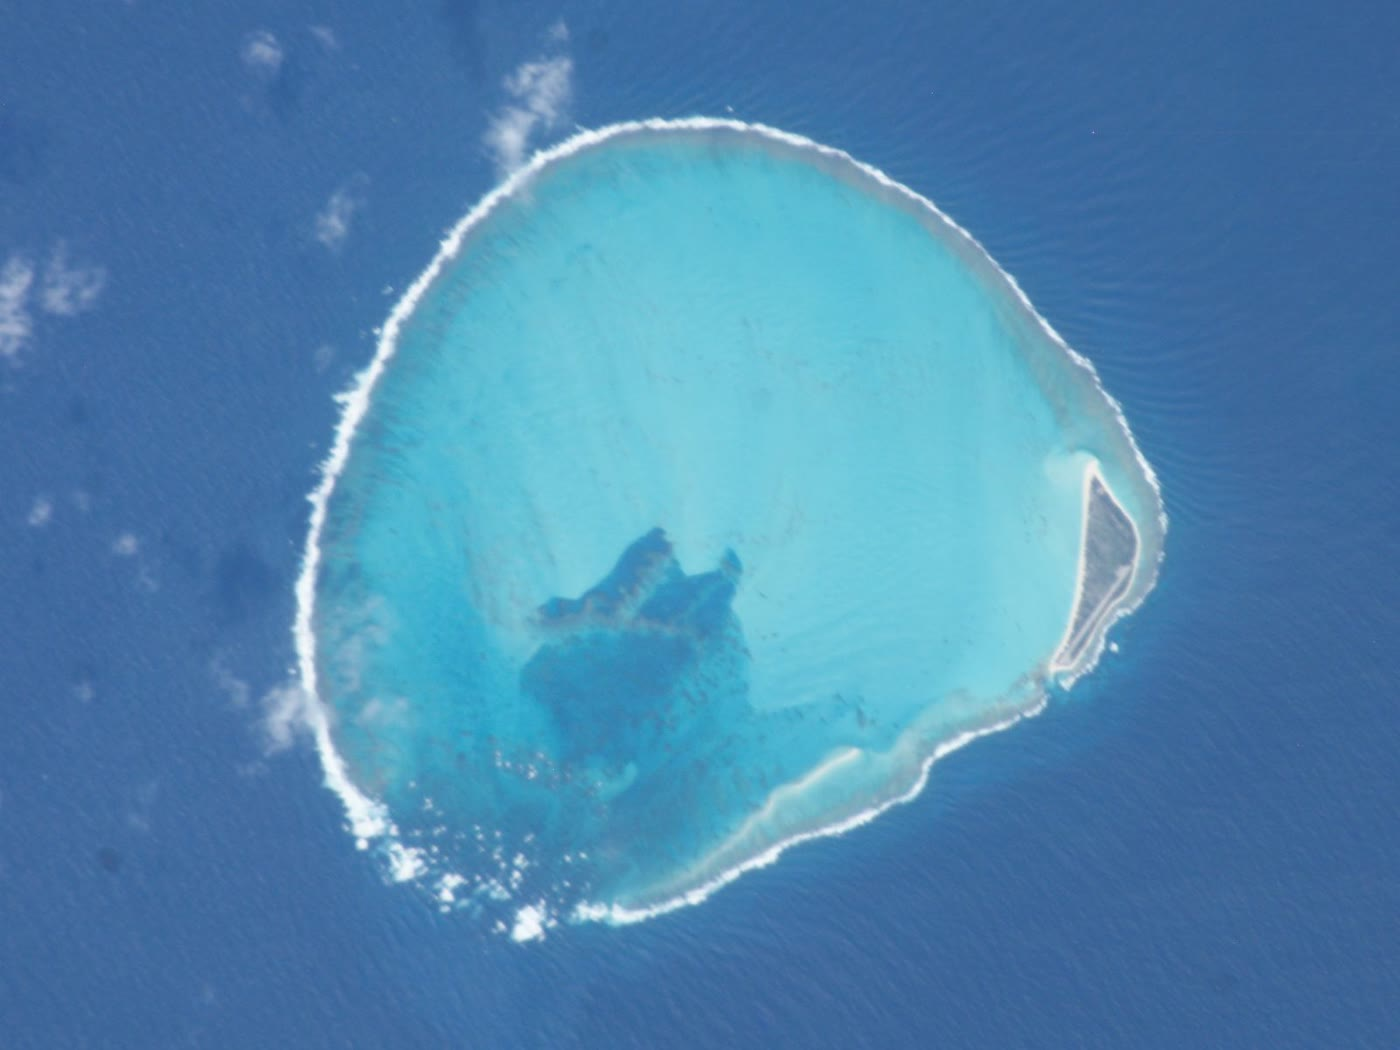
\includegraphics[width=0.52\linewidth]{images/book4/b2-17-kure-atoll.jpg}
\par\smallskip{\small क्योर \omterm{def:b2:oceanic-islands:reefs}{एटॉल}, सबसे उत्तरी प्रवाल \omterm{def:b2:oceanic-islands:reefs}{एटॉल}, जिसका फ़ोटो एक अंतरिक्ष यात्री ने
22 फ़रवरी 2004 को अंतरराष्ट्रीय अंतरिक्ष स्टेशन से लिया। भित्ति का वलय, अधिक से अधिक लगभग दस किलोमीटर
चौड़ा, एक लैगून को घेरता है; एकमात्र स्थायी द्वीप, ग्रीन आइलैंड, किनारे पर (दाएँ) है। NASA,
सार्वजनिक डोमेन, विकिमीडिया कॉमन्स के माध्यम से।}
\end{omfigure}
% ledger: pmnm:kure (6 miles = 9.7 km)

\section{अपरदन, समुद्र-तल और द्वीप का अंत}\label{sec:b2:oceanic-islands:erosion}

धँसते हुए, द्वीप घिसता भी है। ऊँचा द्वीप व्यापारिक पवनों को रोकता है: हवाई ज्वालामुखियों की
पवनमुखी ढलानों पर, कहीं-कहीं एक वर्ष में \qty{9}{m} से अधिक वर्षा होती है।
धाराएँ दस लाख वर्षों से कम में गहरी घाटियाँ काट देती हैं, जैसे हवाई द्वीप पर कोहाला पर।
कुछ बड़े खड़े चट्टानी कगार जिन्हें कभी केवल अपरदन का काम माना गया था, जैसे उत्तरी
मोलोकाई के समुद्री कगार, अब विशाल स्खलनों की शीर्ष-दीवारें माने जाते हैं, जो तब से पीछे कटी हैं। लहरें तट पर आक्रमण करती हैं और
उसके चारों ओर समुद्र-तल पर एक तरंग-घर्षित चबूतरा समतल करती हैं। अपरदन और धँसाव मिलकर समुद्र के ऊपर
ज्वालामुखीय चट्टान का हर निशान लगभग \qty{15}{Myr} में मिटा देते हैं। लगभग उसी आयु के गार्डनर पिनैकल्स
शृंखला का सबसे पुराना द्वीप है जहाँ ज्वालामुखीय चट्टान अब भी पानी के ऊपर खड़ी है। उसके आगे
उत्तर-पश्चिम में केवल रेतीले द्वीप, \omterm{def:b2:oceanic-islands:reefs}{एटॉल} और डूबे ज्वालामुखी हैं।
% ledger: cs14:erosion, cs14:erase

यह सब चलते समय समुद्र-तल स्थिर नहीं रहता। अंतिम हिमनदीय अधिकतम के दौरान वह आज से लगभग
\qty{120}{m} नीचा था। तब किसी द्वीप का तट उसके पार्श्वों पर नीचे था, और जो भित्तियाँ
अब उसे घेरती हैं वे सूखी भूमि थीं। जब बर्फ़ पिघली, समुद्र औसतन हर हज़ार वर्ष \qty{12}{m} उठा, मुख्य विहिमनदन के दौरान,
16.5 से \qty{8.2}{ka} तक। मेल्टवॉटर
पल्स 1A के दौरान वह प्रति वर्ष कम से कम \qty{40}{mm} उठा। धँसते ज्वालामुखी पर भित्ति को दोनों
उत्थानों का अनुसरण करना होता है। हवाई द्वीप के उत्तर-पश्चिमी तट के पास, कम से कम छह डूबी भित्तियाँ
पार्श्व पर एक सीढ़ी बनाती हैं, सबसे पुरानी सबसे गहरी। हर एक तट पर बढ़ी, समुद्र के किसी उत्थान के दौरान
पीछे छूटी, और युवा द्वीप के भारण से नीचे ले जाई गई। जब कोई ज्वालामुखी
लगभग \qty{125}{m}, हिमनदीय समुद्र-तल के परास, से अधिक धँस जाता है, तो वह लहरों में वापस नहीं आएगा।
% ledger: usgs:lgm (Book 1), lambeck14:lgm (Book 2), cs14:erase, cs14:subsidence

मेहराब उलटी दिशा में भी काम कर सकता है। ओआहू नए द्वीपों के भार से उठे उभार पर बैठा है,
और थोड़ा उठा है: अंतिम अंतर्हिमनदीय काल की भित्तियाँ, 133 से \qty{115}{ka} पुरानी, पूरे
द्वीप के चारों ओर दिखती हैं, और लगभग \qty{334}{ka} पुरानी एक भित्ति अब समुद्र-तल से \qty{21}{m} ऊपर खड़ी है। इस प्रकार
किसी \omterm{def:b2:oceanic-islands:stages}{महासागरीय द्वीप} का अंत उसकी चट्टानों और उसकी भित्तियों में लिखा है। लावा उसे बनाता है, स्खलन और
वर्षा उसे काटते हैं, लहरें उसे समतल करती हैं, प्लेट उसे नीचे ले जाती है, और एक भित्ति सतह पर अपना स्थान
बनाए रखती है जब तक ठंडा पानी और उठता समुद्र उसे भी नहीं डुबो देते।
% ledger: cs14:arch

\section*{अभ्यास}\label{sec:b2:oceanic-islands:exercises}

अभ्यासों के आँकड़े, जब तक अन्यथा न कहा जाए: गहराई–आयु नियम $d = \qty{2500}{m} + C\sqrt t$,
$C = \qty{350}{m.Myr^{-1/2}}$ के साथ, $0 \le t \le \qty{70}{Myr}$ के लिए, और $d = \qty{6400}{m} -
\qty{3200}{m}\,e^{-t/62.8}$ \qty{20}{Myr} के आगे; $1~\text{फ़ुट} = \qty{0.3048}{m}$, $1~\text{फ़ैदम}
= \qty{1.8288}{m}$, $1~\text{मील} = \qty{1.609}{km}$; भित्ति-वृद्धि \qty{4.2}{mm.yr^{-1}} तक।

\begin{exercise}[$\star$]\label{exo:b2:oceanic-islands:1}
हर ज्वालामुखी का चरण बताइए: (क) एक \omterm{def:b2:oceanic-islands:seamount}{समुद्री पर्वत} जिसका शिखर समुद्र के \qty{975}{m} नीचे है, और जो
क्षारीय लावा उगलता है; (ख) हॉटस्पॉट के ऊपर एक ज्वालामुखी, जो ऊँची दर से थोलिआइटी लावा उगलता है; (ग) एक
विलुप्त ज्वालामुखी जिसके अंतिम प्रवाह, द्वीप के अधिकांश भाग से अधिक क्षारीय, शील्ड को ढकते हैं; (घ) एक
द्वीप जहाँ, \qty{2}{Myr} की शांति के बाद, कुछ छोटे क्षारीय निकास-छिद्र खुलते हैं; (ङ) एक लैगून के चारों ओर
भित्ति का एक वलय, जिसमें कोई ज्वालामुखीय चट्टान दिखाई नहीं देती।
\end{exercise}

\begin{exercise}[$\star$]\label{exo:b2:oceanic-islands:2}
एक ज्वालामुखी \qty{9}{Myr} पुरानी प्लेट पर बना है। (क) उसके आसपास समुद्र-तल कितना गहरा है? (ख) जब
प्लेट \qty{25}{Myr} पुरानी होगी, तब तक वह कितना धँस चुका होगा? (ग) तब वह किस दर से धँस रहा है?
\end{exercise}

\begin{exercise}[$\star$]\label{exo:b2:oceanic-islands:3}
मुख्य हवाई द्वीपों के आसपास पिछले \qty{5}{Myr} में सत्रह बड़े स्खलन बने, और
हवाई कटक के अनुदिश \qty{30}{Myr} में सत्तर। (क) हर स्थिति में दो स्खलनों के बीच का माध्य अंतराल
निकालिए। (ख) दोनों वास्तविक अंतराल की केवल ऊपरी सीमाएँ क्यों हैं?
\end{exercise}

\begin{exercise}[$\star$]\label{exo:b2:oceanic-islands:4}
एनीवेटक पर, एक बोरहोल में बेसाल्ट 4,158 फ़ुट पर और दूसरे में कठोर आधारशैल 4,610 फ़ुट पर मिला;
चूना-पत्थर के आधार पर के भित्ति-प्रवाल 150 फ़ुट से अधिक गहराई पर नहीं रहते। (क) तीनों
गहराइयों को मीटर में बदलिए। (ख) पैरी द्वीप के नीचे ज्वालामुखी का शीर्ष, उस पर पहली भित्ति उगने के बाद से,
कम से कम कितना धँसा है? (ग) चूना-पत्थर का आधार इओसीन है, अतः कम से कम
\qty{33.9}{Myr} पुराना। धँसाव की अधिकतम संभव माध्य दर क्या है?
\end{exercise}

\begin{exercise}[$\star\star$]\label{exo:b2:oceanic-islands:5}
(क) 4, 25 और \qty{49}{Myr} पुरानी प्लेटों पर बने द्वीपों के तापीय धँसाव की दर, \unit{m} प्रति \unit{Myr} में और \unit{mm.yr^{-1}} में,
निकालिए। (ख) कोई उत्पादक भित्ति इनमें से सबसे तेज़ से
कितने गुना तेज़ बढ़ सकती है? (ग) और हवाई द्वीप के पास का भारण चरण,
प्रति हज़ार वर्ष \qty{2.6}{m}, कितने गुना तेज़ है?
\end{exercise}

\begin{exercise}[$\star\star$]\label{exo:b2:oceanic-islands:6}
(क) घातांकी नियम के साथ, \qty{100}{Myr} पुरानी प्लेट पर धँसाव की दर, \unit{m}
प्रति हज़ार वर्ष में, निकालिए, और उसकी तुलना हवाई कटक के अनुदिश मापी गई प्रति हज़ार वर्ष \qty{0.01}{m} से कीजिए।
(ख) किस प्लेट-आयु पर दर ठीक \qty{10}{m.Myr^{-1}} है? (ग) जाँचिए कि
\qty{25}{Myr} पुरानी प्लेट के लिए दोनों नियम लगभग समान गहराई देते हैं।
\end{exercise}

\begin{exercise}[$\star\star$]\label{exo:b2:oceanic-islands:7}
हवाई भित्तियाँ अपने ज्वालामुखी के जन्म के लगभग \qty{33}{Myr} बाद डूबती हैं, और ज्वालामुखी-क्रिया
शृंखला के अनुदिश \qty{8.6}{cm.yr^{-1}} से खिसकती है। (क) जब किसी द्वीप की भित्ति डूबती है, तब वह हॉटस्पॉट से
कितनी दूर होता है? (ख) मिडवे \qty{27.7}{Myr} पुराना \omterm{def:b2:oceanic-islands:reefs}{एटॉल} है: क्या यह संगत है कि उसमें अब भी एक
जीवित भित्ति है? (ग) क्योर मिडवे से 55 मील आगे है। उसकी आयु का अनुमान लगाइए, और बताइए कि क्या वह
\omterm{def:b2:oceanic-islands:darwin-point}{डार्विन बिंदु} के निकट है।
\end{exercise}

\begin{exercise}[$\star\star$]\label{exo:b2:oceanic-islands:8}
नुउआनु \omterm{def:b2:oceanic-islands:collapse}{मलबा-हिमस्खलन} में, टस्कलूसा \omterm{def:b2:oceanic-islands:seamount}{समुद्री पर्वत} लगभग \qty{30}{km} लंबा,
\qty{17}{km} चौड़ा और कम से कम \qty{2}{km} ऊँचा एक खंड है। (क) इन विमाओं वाले बक्से का आयतन
कितना होगा? और उसी आधार और उसी ऊँचाई वाले पिरामिड का? (ख) किलाउआ के आयतन,
\qty{10000}{km^3}, से तुलना कीजिए। (ग) हिमस्खलन \qty{23000}{km^2} ढकता है। यदि वह औसतन
\qty{100}{m} मोटा होता (एक मान्यता: ओआहू से दूर उसकी मोटाई ठीक से ज्ञात नहीं), तो उसका
आयतन कितना होता?
\end{exercise}

\begin{exercise}[$\star\star$]\label{exo:b2:oceanic-islands:9}
हवाई द्वीप के पास पार्श्व ज्वालामुखी के भार के नीचे प्रति हज़ार वर्ष \qty{2.6}{m} धँसता है।
(क) किसी तटरेखा को \qty{1}{km} डुबोने में कितना समय लगता है? (ख)
\qty{4.2}{mm.yr^{-1}} से बढ़ती एक भित्ति इस पार्श्व पर है। क्या समुद्र-तल स्थिर रहने पर वह साथ बनी रहती है? (ग) मुख्य
विहिमनदन के दौरान, 16.5 से \qty{8.2}{ka} तक, समुद्र औसतन \qty{12}{mm.yr^{-1}} उठा। यदि भित्ति
सतह से आरंभ हुई थी, तो अंत में उसका शीर्ष कितना गहरा है? (घ) यही, किसी ऐसे पुराने ज्वालामुखी पर की भित्ति के लिए
जो अब नहीं धँसता।
\end{exercise}

\begin{exercise}[$\star\star\star$]\label{exo:b2:oceanic-islands:10}
(क) दिखाइए कि, किसी नियत अंतराल $\Delta$ में, मूल नियम के अनुसार प्लेट जितनी पुरानी हो, द्वीप उतना ही कम
धँसता है। (ख) \qty{20}{Myr} में धँसाव निकालिए, कटक पर जन्मे द्वीप के लिए और
\qty{50}{Myr} पुरानी प्लेट पर जन्मे द्वीप के लिए। (ग) कटक के नीचे की प्लेट बहुत गर्म होती है, और मूल नियम
$t = 0$ पर अनंत दर देता है। क्या यह किसी परिमित अंतराल में धँसाव के लिए समस्या है? समझाइए।
\end{exercise}

\begin{exercise}[$\star\star\star$]\label{exo:b2:oceanic-islands:11}
एक \omterm{def:b2:oceanic-islands:reefs}{एटॉल} \qty{30}{m.Myr^{-1}} से धँसता है, और समुद्र-तल हिमयुगों के साथ लगभग \qty{120}{m}
झूलता है, लगभग \qty{100}{kyr} के चक्रों में। (क) एक चक्र में \omterm{def:b2:oceanic-islands:reefs}{एटॉल} कितना धँसता है? (ख) किसी
हिमनदीय निम्न-स्तर पर, \omterm{def:b2:oceanic-islands:reefs}{एटॉल} का शीर्ष समुद्र से कितना ऊपर खड़ा होता है? तब भित्ति-चट्टान का क्या होता है?
(ग) \omterm{def:b2:oceanic-islands:reefs}{एटॉल} को पूरे \qty{120}{m} धँसने में कितने चक्र लगते हैं?
(घ) एनीवेटक के बोरहोलों में मिले निक्षालित मंडलों की व्याख्या कीजिए, और बताइए कि
\cref{prop:b2:oceanic-islands:cap} लंबी अवधि में फिर भी टोपी की मोटाई क्यों देता है।
\end{exercise}

\begin{exercise}[$\star\star\star$]\label{exo:b2:oceanic-islands:12}
एक \omterm{def:b2:oceanic-islands:reefs}{एटॉल} तब डूबता है जब उसकी प्लेट \qty{50}{Myr} पुरानी है: उसकी भित्ति पीछे छूटती है और उसका शीर्ष
सबसे गहरे प्रवाली शैवालों की वृद्धि-सीमा, समुद्र के \qty{150}{m} नीचे, पर समाप्त होता है। (क) घातांकी
नियम के साथ, प्लेट के \qty{120}{Myr} पुरानी होने से पहले वह और कितना धँसता है? (ख) तब \omterm{def:b2:oceanic-islands:seamount}{गयो} का
शीर्ष कितना गहरा है? (ग) एनीवेटक के पास एक \omterm{def:b2:oceanic-islands:seamount}{गयो} का शीर्ष 700 फ़ैदम पर है। रूपांतरित कीजिए, और तुलना कीजिए।
(घ) दो कारण बताइए कि कोई वास्तविक \omterm{def:b2:oceanic-islands:seamount}{गयो} इस अनुमान से गहरा या उथला क्यों हो सकता है।
\end{exercise}

\begin{problem}[{सप्ताहांत समस्या --- ज्वालामुखी से एटॉल तक}]\label{pb:b2:oceanic-islands:1}
कल्पित पेट्रेल द्वीप \qty{10}{Myr} पुरानी प्लेट पर एक हॉटस्पॉट के ऊपर जन्मता है। उसका ज्वालामुखी
\qty{50}{km} आधार-त्रिज्या का एक शंकु है। जब उसकी वृद्धि समाप्त होती है, उसका शिखर समुद्र-तल से
\qty{1000}{m} ऊपर खड़ा होता है। उसकी अंतिम ज्वालामुखीय चट्टान \qty{12}{Myr} बाद समुद्र-तल के नीचे लुप्त हो जाती है। फिर एक भित्ति
अपना शीर्ष समुद्र-तल पर तब तक रखती है जब तक प्लेट \qty{70}{Myr} पुरानी न हो जाए, जब \omterm{def:b2:oceanic-islands:reefs}{एटॉल}
\omterm{def:b2:oceanic-islands:darwin-point}{डार्विन बिंदु} पार करता है। अभ्यासों का गहराई–आयु नियम (\qty{70}{Myr} तक मूल नियम, उसके आगे
घातांकी नियम), \qty{4.2}{mm.yr^{-1}} की भित्ति-वृद्धि, और अध्याय के आँकड़े उपयोग कीजिए।
प्रश्न 8 से 10 को छोड़कर समुद्र-तल को स्थिर माना जाता है। गहराइयों को मीटर तक पूर्णांकित कीजिए।

\noindent\textbf{भाग I --- वृद्धि।}
\begin{enumerate}
  \item जहाँ पेट्रेल जन्मता है, वहाँ समुद्र-तल कितना गहरा है?
  \item जब उसकी वृद्धि समाप्त होती है, उस तल से ज्वालामुखी की ऊँचाई क्या है, भार के नीचे
        तल के धँसने की उपेक्षा करते हुए?
  \item शंकु का आयतन निकालिए।
  \item यदि उसका \qty{85}{\percent} \qty{1}{Myr} के \omterm{def:b2:oceanic-islands:stages}{शील्ड चरण} के दौरान उगला गया, तो
        उद्गार की माध्य दर क्या थी? आज किलाउआ की आपूर्ति, लगभग
        \qty{0.1}{km^3} प्रति वर्ष, से तुलना कीजिए।
  \item कितने पेट्रेल मिलकर एक माउना लोआ, \qty{95600}{km^3}, बनाएँगे?
  \item कौन-से लावा, थोलिआइटी या क्षारीय, शंकु का अधिकांश भाग बनाते हैं? कौन-से उसे ढकते हैं?
\end{enumerate}

\noindent\textbf{भाग II --- भारण और डूबी भित्तियाँ।}
\begin{enumerate}[resume]
  \item अपनी वृद्धि के दौरान, भार युवा द्वीप को \qty{1}{km} \qty{1}{Myr} में धँसाता है। माध्य
        दर क्या है, और हवाई द्वीप के पास मापी गई प्रति हज़ार वर्ष \qty{2.6}{m} से
        उसकी तुलना कैसी है?
  \item इस चरण के दौरान तट पर एक भित्ति बढ़ती है, समुद्र-तल स्थिर रहते हुए। क्या वह साथ बनी रहती है, और
        कितने अंतर से?
  \item फिर समुद्र-तल \qty{12}{mm.yr^{-1}} से उठता है। भित्ति हर वर्ष कितनी पीछे
        छूटती है?
  \item उसका शीर्ष \qty{150}{m}, सबसे गहरी वृद्धि-सीमा, तक पहुँचने में कितना समय लगता है? इससे
        द्वीप के पार्श्व पर क्या बचता है?
\end{enumerate}

\noindent\textbf{भाग III --- धँसाव और अपरदन।}
\begin{enumerate}[resume]
  \item जब तक उसकी अंतिम ज्वालामुखीय चट्टान लुप्त होती है, प्लेट तब
        \qty{22}{Myr} पुरानी होने पर, पेट्रेल कितना धँस चुका है?
  \item शिखर के \qty{1000}{m} में से कितना अपरदन ने हटाया, और किस माध्य दर से?
  \item जब उसकी वृद्धि समाप्त होती है, और जब उसका शिखर लुप्त होता है, तब पेट्रेल किस दर से धँस रहा है?
  \item तब उसके आसपास समुद्र-तल कितना गहरा है?
  \item उसे लगे \qty{12}{Myr} की तुलना हवाई द्वीपों के \qty{15}{Myr} से कीजिए। एक
        कारण बताइए कि कोई ऊँचा हवाई द्वीप अधिक समय तक क्यों टिकता है।
  \item वर्षा और नदियों के अतिरिक्त दो प्रक्रियाएँ बताइए जो समुद्र-तल से ऊपर के द्वीप को हटाती हैं।
  \item शिखर लुप्त होने से कुछ पहले पेट्रेल को भित्ति का कौन-सा रूप घेरता है?
\end{enumerate}

\noindent\textbf{भाग IV --- एटॉल और गयो।}
\begin{enumerate}[resume]
  \item जब प्लेट \qty{70}{Myr} पुरानी है, तब भित्ति-टोपी कितनी मोटी है?
  \item इसके लिए भित्ति-वृद्धि की कौन-सी माध्य दर चाहिए थी? वह उस वृद्धि से कितने गुना छोटी है
        जो भित्ति प्राप्त कर सकती थी?
  \item टोपी की तुलना एनीवेटक के नीचे बेसाल्ट की गहराई से कीजिए।
  \item जब \omterm{def:b2:oceanic-islands:reefs}{एटॉल} \omterm{def:b2:oceanic-islands:darwin-point}{डार्विन बिंदु} पार करता है, तब उसके आसपास समुद्र-तल कितना गहरा है?
  \item घातांकी नियम के साथ, प्लेट के \qty{120}{Myr} पुरानी होने से पहले डूबा \omterm{def:b2:oceanic-islands:reefs}{एटॉल} और कितना
        धँसता है?
  \item यदि डूबते समय भित्ति का शीर्ष \qty{150}{m} पर रुका, तो तब \omterm{def:b2:oceanic-islands:seamount}{गयो} का शीर्ष कितना
        गहरा है?
  \item सारांश में: पेट्रेल \omterm{def:b2:oceanic-islands:reefs}{एटॉल} की भित्ति-टोपी कितनी मोटी है?
\end{enumerate}
\end{problem}
